\section{Introduction}
\label{sec:introduction}
% state the learning objective 
The objective of this laboratory assignment is to study a circuit containing a
AC voltage source $v_s$, seven resistors, a voltage-controlled current source $I_b$, a capacitor $C$
and a current-controlled voltage source $V_d$. The components of this circuit are distribuited 
by 4 elementary meshes and 8 nodes, as seen in Figure~\ref{fig:circuit}. 

In order to analyse the circuit, the following data were obtained by running the supplied Python script: 

\textit{Units for the values:} V, A, F, Ohm and S\par
\textit{Values:}
\begin{table}[H]
  \centering
  \begin{tabular}{|l|r|}
    \hline    
    $R_{1a}$ & 1.000000e+03 Ohm \\ \hline
$R_{1b}$ & 1.000000e+04 Ohm \\ \hline
$R_{1}$ & 9.090909e+02 Ohm\\ \hline
$R_{2}$ & 1.000000e+03 Ohm \\ \hline
$R_{3a}$ & 1.000000e+05 Ohm \\ \hline
$R_{3b}$ & 1.000000e+05 Ohm \\ \hline
$R_{3c}$ & 1.000000e+05 Ohm \\ \hline
$R_{3}$ & 1.500000e+05 Ohm \\ \hline
$R_{4a}$ & 1.000000e+03 Ohm \\ \hline
$R_{4b}$ & 1.000000e+04 Ohm \\ \hline
$R_{4}$ & 9.090909e+02 Ohm \\ \hline
$C_{1}$ & 2.200000e-07 F \\ \hline
$C_{2a}$ & 2.200000e-07 Ohm \\ \hline
$C_{2b}$ & 2.200000e-07 Ohm \\ \hline
$C_{2}$ & 1.100000e-07 F \\ \hline

  \end{tabular}
  \caption{Data Table}
  \label{tab:datatab}
\end{table}

In Section~\ref{sec:analysis}, a theoretical analysis of the circuit, 
performed on Octave, is presented. In Section~\ref{sec:simulation}, the 
circuit is analysed by simulation, using NGSpice, and the results are compared to 
the theoretical results obtained in Section~\ref{sec:analysis}. The conclusions 
of this study are outlined in Section~\ref{sec:conclusion}.

\begin{figure}[H] \centering
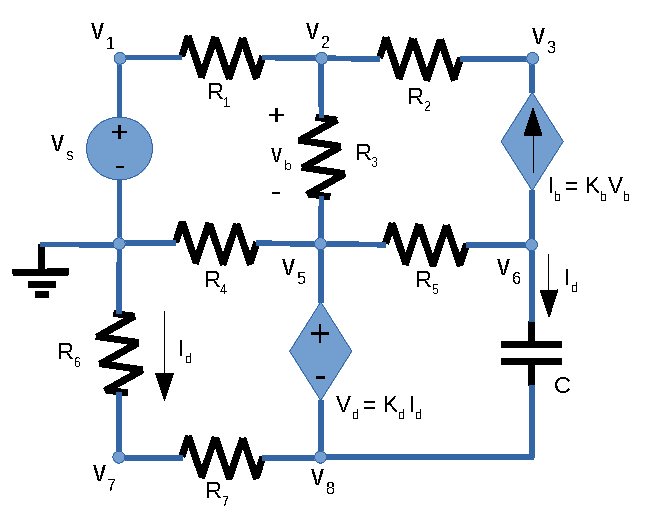
\includegraphics[width=0.4\linewidth]{circuit.pdf}
\caption{Circuit which will be analysed during this laboratory assignment.}
\label{fig:circuit}
\end{figure}

